%Texlive-full Version 3.141592-1.40.3 (Web2C 7.5.6)
%TexStudio Version 2.7.0

\documentclass[a4paper,10pt]{article}
\usepackage[utf8]{inputenc}
\usepackage{graphicx}

\usepackage{lmodern}
\usepackage[a4paper]{geometry}

\usepackage{hyperref}
\usepackage{enumitem}
% \usepackage{nomencl}\makenomenclature

\usepackage{amsmath}
\usepackage{amssymb}
\usepackage{amsthm}

\usepackage{pstricks}
\usepackage{pst-node}
\usepackage{color}
\usepackage[ddmmyyyy]{datetime} 


\newcommand{\E}{\mathbb{E}}
\newcommand{\Proba}{\mathbb{P}}
\newcommand{\F}{\mathcal{F}}
\newcommand{\Bt}{B_t}
\newcommand{\DtT}{D(t,T)}
\newcommand{\RtT}{R(t,T)}
\newcommand{\PtT}{P(t,T)}
\newcommand{\PtS}{P(t,S)}
\newcommand{\LtT}{l(t,T)}
\newcommand{\YtT}{Y(t,T)}
\newcommand{\ftT}{f(t,T)}
\newcommand{\tautT}{\tau(t,T)}
\newcommand{\inttT}{\int_t^T}
\newcommand{\intt}{\int_0^t}
\newcommand{\FuncExp}{\text{exp}}
\newcommand{\FuncLn}{\text{ln}}
\newcommand{\Discount}[2]{e^{-\int_{#1}^{#2}r_u du} }
\newcommand{\bl}[1]{{\scshape  #1}}


\newcommand{\Ti}{T_{i}}
\newcommand{\Tj}{T_{j}}
\newcommand{\Ta}{T_{\alpha}}
\newcommand{\Tb}{T_{\beta}}
\newcommand{\Tii}{T_{i+1}}
\newcommand{\Pti}{P(t,T_{i})}
\newcommand{\Ptii}{P(t,T_{i+1})}
\newcommand{\Lti}{L(t,\Ti,\Tii)}
\newcommand{\Lit}{L_{i}(t)}
\newcommand{\muit}{\mu_i(t)}
\newcommand{\sigmait}{\sigma_i(t)}
\newcommand{\Wit}{W^{\Tii}(t)}
\newcommand{\Wnt}{W^{T_{N+1}}(t)}
\newcommand{\Ltj}{L(t,\Tj,\Tj)}
\newcommand{\Ljt}{L_{j}(t)}
\newcommand{\sigmajt}{\sigma_j(t)}
\newcommand{\ZCi}{ZC_{i}}
\newcommand{\ZCii}{ZC_{i+1}}
\newcommand{\Numi}{Num_{i}}
\newcommand{\Numii}{Num_{i+1}}

\newcommand{\Sab}{S_{\alpha,\beta}}
\newcommand{\Cab}{C_{\alpha,\beta}}
\newcommand{\Wab}{W_{\alpha,\beta}}
\newcommand{\sigmaab}{\sigma_{\alpha,\beta}}
\newcommand{\rhoij}{\rho_{ij}}
\newcommand{\Eab}{\mathbb{E}^{\alpha,\beta}}

\newcommand{\todo}[1]{\begin{center}\color{red} TODO : #1\end{center}}

\begin{document}
\begin{titlepage}
%%%%%%%%%%%%%%%%%%%%%%%%%%  LOGO  %%%%%%%%%%%%%%%%%%%%%%%%%%%%%%%%%%%%%%%%%
\begin{center}
\begin{pspicture}(-7,0)(7,2)
%\psline(-7,0)(7,2)
\rput(-9,2){\href{http://www.univ-paris-diderot.fr/english/sc/site.php?bc=accueil&np=accueil&g=m}{
\includegraphics[scale=1.2]{logo_p7}}}
\rput( -3.5,1){\href{hhttp://www.lunalogic.com/en/}{
\includegraphics[scale=0.4]{logo_luna}}}
\rput(4,2){\href{https://masterfinance.math.univ-paris-diderot.fr/}
	    {	\begin{tabular}{l}
		\resizebox{4cm}{0.6cm}{M2MO} \\
		\resizebox{6cm}{0.5cm}{DEA Laure Elie}  
		\end{tabular}
	    }
}

\rput(3,-0.5){
\begin{tabular}{ll}
Tutors                                                                  &              \\ 
\href{mailto:revierdenord@gmail.com}{\textbf{Yuan LI} }                 &(Lunalogic)  \\
\href{mailto:scotti@math.univ-paris-diderot.fr}{\textbf{Simone SCOTTI}} &(Paris 7)  
\end{tabular}	    
}
%\psline(-7,0)(7,2)
\end{pspicture}
\end{center}



%%%%%%%%%%%%%%%%%% DOCUMENT TITLE %%%%%%%%%%%%%%%%%%%%%%%%%
\vspace{2cm}

\begin{center}
\resizebox{14cm}{0.8cm}{Libor Market Model}
\end{center}
%%%%%%%%%%%%%%%%%% DOCUMENT TITLE %%%%%%%%%%%%%%%%%%%%%%%%%
\begin{center}
\huge{ Version : \today }
\end{center}


\begin{center}
\href{mailto:chithanhnguyen.math@gmail.com}{\LARGE{\textbf{Chi Thanh NGUYEN}}}
\end{center}



\vfill
\begin{abstract}
Master M2MO (\textbf{Laure Elie}'s DEA) is one of the most prestige Financial Engineering Master program in France, and Europe. At the end of this Master program, a minimum 6 months internship is required in order to assimilate partly the whole theoretical knowledge acquired from the Master. The intership for me take place at Lunalogic, a consulting \& service enterprise for banks and insurances. The main objective at Lunalogic is to have internal libraries studying the financial modelling, with advanced mathematical tools implemented in C++ or C\#. However this project is at its own begining phase, i.e models and tools are usually build independantly in form of prototyping (sub projects), ensuring a minimum of accuracy and code qualities. At a second phase, every prototype should be refactorized and integrate into a whole common library. In the internship at Lunalogic, we continu the work of ~\cite{THAI2013} and use the book  ~\cite{BRIGO2006} ~\cite{BRIGO2005}
\end{abstract}
\end{titlepage}


\tableofcontents
\newpage

%%%%%%%%%%%%%%%%%%%%%%%%%%%%%%%%%%%%%%%
\newpage
\section{About Lunalogic}
\begin{tabular}{llll}
Position          &            Name              & Contact                        &Telephone      \\
Exec Director     & Fathia Rahmani               & fathia.rahmani@lunalogic.com   &               \\
HR   Director     & Isabelle Marouby             & isabelle.marouby@lunalogic.com &06.51.44.06.78 \\
Quant Consultant  & Yuan Li                      & revierdenord@gmail.com         &06.52.17.69.75 \\    
Tech. support     & Fastah Rahmani               & fastah.rahmani@gmail.com       &               \\ 
Bloomberg supp.   & Giulio D'Ambrosio            & gdambrosio3@bloomberg.net      &+442070733101  \\
\end{tabular}

\newpage
\section{The Market Model}
The aim of market model is to give a model that well price a set of basic instruments. In the LMM case study, the aim is to give a good pricing tool for plain vanilla products, such as Caps, Floors and Swaptions. In this section, firstly show the idea of numeraire change, this idea lies the model and the well-etablished pricing tool for simple instruments. 
\subsection{Numeraire change and market models}
The two important numeraire changes that make the market model of this project are inspired from the Caplet and Swaption Black \& Scholes frameworks. 
\paragraph{ Caplet and forward measure } is an option on interest rate derivative. Caplet is analyzed as a european call option, with maturity time $T_1$ and pay at time $T_2$ for a certain strike $K$. The payment of such an option at time $T_2$ is obsevable at time $T_1$ and worth
\[
\text{price}(T_1) = \tau(T_1,T_2)( L(T_1;T_1,T_2) - K )^+ 
\] 
where $L(T_1,T_1,T_2)$ is the observed Libor at time $T_1$. This payoff at the present time can be obtainted by discounting 
\[
\text{price}(0) = \mathbb{E}^{B}\left[ \frac{B(0)}{B(T_2)} \tau(T_1,T_2)( L(T_1;T_1,T_2) - K )^+  \right]
\]
with $B(t)$ the money market account. Since the zerocoupond $P(t,T_2)$ is a tradable instrument, and always have positive values, one can change the numeraire, and the pricing formula becomes
\[
\text{price}(0) = \tau(T_1,T_2)P(0,T_2) \mathbb{E}^{T_2}\left[ ( L(T_1;T_1,T_2) - K )^+  \right]
\]
Note that by using $P(t,T_2)$ as numeraire, $\mathbb{E}^{T_2}$ is defined as $T_2$-forward measure, and under such probability, the forward rate follow a martingale, i.e
\[
\frac{dL(t;T_1,T_2)}{L(t;T_1,T_2)} = v^{T_2}dW^{T_2}
\hspace{2cm}
t\leq T_1 < T_2
\]
\paragraph{ Swaption and swap measure } is the option to enter into a interest rate swap. As for swap interest rate, swaption contract is settled on a set of payment dates $\Ta.. T_i.. \Tb$ where $\Ta$ and $\Tb$ are start and end of swap instrument. The swaption's maturity date is the swap's start date $\Ta$. The price value of such an option is caculable at time $\Ta$ by discounting
\[
\text{price}(\Ta) = \left[ \Sab(\Ta) - K \right]^+ \Cab(\Ta)
\hspace{1cm}
\Cab(t) = \sum^{\beta-1}_{\alpha} \tau_i \Ptii 
\]  
Where $\Cab(t)$ is the swap's annuity measure at time $t$. This is simply the payment sum of the fix leg on a swap configuration. Note that annuity is indeed a tradable product, as a sum of zerocoupons, always have positive value, so those can be used as numeraire. By the same way as discounting the caplet price, the present value of swaption is
\[
\text{price}(0) = \mathbb{E}^{B}\left[ \frac{B(0)}{B(T_2)} (\Sab(\Ta) - K )^+ \Cab(\Ta)  \right]
\]
and by change to numeraire $\Cab(t)$, under the associated probability $\Eab$
\[
\text{price}(0) = \Cab(0) \Eab \left[ (\Sab(\Ta) - K )^+  \right]
\]
Since the numeraire change framework ensure the martingale properties, the swap interest rate $\Sab$ under the measure $\Eab$ follows the martingale, in the way that it can be modelled by equation
\[
\frac{d\Sab(t)}{\Sab(t)} = \sigmaab(t) d\Wab(t)
\]
\paragraph{} These two pricing approachs introduce to two different ideas of modelling for differents basic instrument. That also show the incompatibilities issues of these two derivative's familly. The evidence come from the fact that the measure $\mathbb{E}^{T_2}$ associated to the numeraire $P(t,T_2)$ is different to the measure $\Eab$ associated to the numeraire $\Cab(t)$.   

\subsection{Lognormal Forward Libor model}
As its name, the Lognormal Forward Libor Model ( or simply Libor Market Model), is the model that describ the dynamic of forward rate. The idea is if one know all values of forward rate, one can calculate easily the price of many related fixed income derivative as caps, floors, swaptions ... {\color{red} some more blah blah for model :}
\paragraph{Model configuration} is firstly defined by a timeline setting. Although the mathenatical definition of forward rate is a continuous functions, its implementation can only be done through a discrete configuration. There are different choice for time discretizetion, more or less dense, but we choose the simplest one : the dates coincide with the settlement date of Libor. In the US market, that is every 3MO, in the European market, that is every 6MO. By giving a maximum horizon, we discretize our times to a set of date $\xi=\left\{T_0, .. T_i, ..T_N \right\}$ \footnote{In the Bloomberg terminal one can get a yield curve for 50YR Max. There are no sens to define a timeline longer than 50YR}. After defining the timeline, we give some conventions for related values.
\begin{itemize}
 \item horizon  = N
 \item Timeline $T_i$ , i = 0,1, .... N+1, $T_0 = 0$, Timeline size = N+2
 \item Time Fractions $\tau_i = \Tii-\Ti$, i=0,1,... N. 
 \item The i-th Libor value at time $t$ : $\Lit = \Lti$, Number of LIBORs = N+1
\end{itemize}
This timeline discretization at the first part facilite the whole implementation. Henceforth, every calculated values can be stored in a container, and every calculation loop iterate through time indices instead of time value.   
\begin{figure}[h]
\begin{center}
\begin{pspicture}(-7,-3)(7,4)
%% Reference for Picture
%\psline[linewidth=0.1pt,linecolor=gray](-7,-3)(7,4)
%\rput(-2,-2){(-2,-2)}\rput(3,3){(3,3)}\rput(0,0){(0,0)}
%%%%%%%%%%%%%%%%%%%%%%%%%%%%%%%%%%%%%%%%%%%%%%%%%%%%%%%%%%%%%%%%%%%%
%% Draw libor matrix
\psgrid[gridwidth=0.01pt,gridcolor=lightgray,subgriddiv=2,subgridwidth=0.1pt,subgridcolor=lightgray,gridlabels=0](-2,-2)(3,3)          % set grid for vol matrix
%% set horizon label for vol matrix
\rput(-2,3.1){$\scriptstyle{T_0}$}
\rput(-1.5,3.1){$\scriptstyle{T_1}$}
\rput(0,3.1){$\scriptstyle{\Tj}$}
\rput(3,3.1){$\scriptstyle{T_{N}}$} 
%% set vertical label for vol matrix
\rput(-2.5,2.5){$L_{1}(.)$}
\rput(-2.5,2){$L_{2}(.)$}
\rput(-2.5,0){$L_i(.)$}
\rput(-2.5,-2){$L_{N}(.)$}     
\rput(0,0){$\bullet$}\rput(0.5,0.2){$L_{i}(\Tj)$}
%%
%%%%%% draw the lower triangular part of libor matrix
{
\pspolygon[fillstyle=crosshatch,hatchcolor=gray,hatchwidth=0.1pt,hatchsep=1pt,linestyle=none](-2,3)(-2,-2)(3,-2)
}
\end{pspicture}
\end{center}
\caption{\label{libor_matrix} Lower triangular matrix used for storage Libor values}
\end{figure}

\begin{itemize}
 \item A LIBOR is a process that is identified by its maturity time $T_i$, its values is calculated at every time $T_j\leq T_i$. Thus libors values can be stored in a lower triangular matrix $(N+1)\times(N+1)$, where $(i,j)$ indices get the $i$-th Libor at time $T_j$
 \item A Vanilla Swaption is an instrument firstly defined by a pair of indices $(\alpha,\beta)$, meaning the expiry time $\Ta$ and tenor $\Tb-\Ta$. Note that $\Tb$ is the end date of the swaption and $\Ta<\Tb$ has to be ensured
 \item The deterministic volatility is defined in our implementation as piecewise volatilities. It is defined by three lower triangular matrix $h,g$ and shift matrix, all of same size as Libor matrix. Note that the first row and first column of volatility matrices are not used since at time zero, all libor are know by extracting data from the quoted market.
 \item correlation model is a little more complicated, but we can say that the correlation between two libor $\Lit$,$\Ljt$ is modelled by a correlation value $\rhoij$. Roughly speaking, it is also a symetric matrix of size $(N+1)\times(N+1)$.   
\end{itemize}
\paragraph{Forward libor dynamic } is described by lognormal processes. For every settlement date $\Ti$, under the numeraire $\Ptii$, the associated forward libor $\Lti$ follow the dynamic
\[
\frac{d\Lit}{\Lit} = \sigmait d\Wit
\]
After translating the brownian $N-i$ times, under the numeraire $P(t,T_{N+1})$, for every date $\Ti$, the dynamic of the forward libor remain a lognomal process, but this time with drift under the terminal probability  
\[
\frac{d\Lit}{\Lit} = \muit + \sigmait d\Wnt
\hspace{1cm}
d\Wnt d\Wnt = \rho dt
\]
Since the Brownian is now the unique one under the terminal measure, we can ommit the subscript for simplify the notations. Furthurmore, we introduce other indices used for indicating the multidimentional brownian and its correlation. The forward libor dynamic finally become
\[
\frac{d\Lit}{\Lit} = \muit + \sigmait \rho^{\frac{1}{2} } dW(t)
\]
\paragraph{Correlation} should be a function of time. But a first implementation can simplify by a function constant in time. ~\cite{BRIGO2006}p.247 mention that the correlation has to satisfy some financial feature
\begin{itemize}
\item $0 \leq \rhoij \leq 1 $ for all $i,j$, a symetric matrix
\item $\rho_{kk} = 1 $ for all $k$ 
\item When moving away from the prinicipal diagonal, $\rhoij$ decrease 
\item When moving along a sub-diagonal from top to bottom, $\rhoij$ increase 
\end{itemize} 
There are several way of modelling the correlation. The essential use should be a parameterized one
\[
\rhoij = e^{- \beta \frac{ |i-j| }{(i+j)^{\alpha}}}
\]
\paragraph{Volatility and time homogeneity feature} is proposed in ~\cite{REBONATO2002}. A parameterized volatility model aslo known as "abcd" volatility having a perfect time homogeneuous properties is modelled as below
\[
h(T-t) = (a + b(T-t)) e^{-c(T-t)} + d
\]
\begin {figure}[h]
\begin{center}
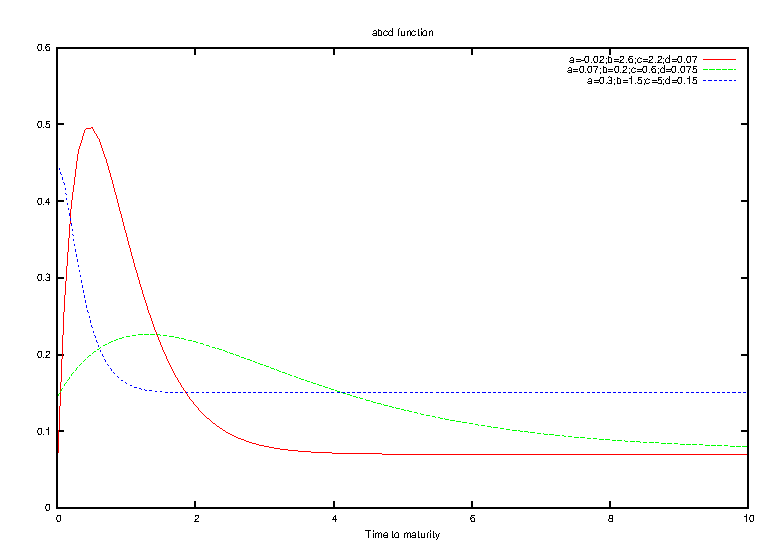
\includegraphics[scale=1.0]{gnuplot_abcdFunction}
\end{center}
\end {figure}







\subsection{Approximation Rebonato's formula}
As we have seen the issue from incompatibility of forward swap model and the forward rate model. In ~\cite{JACKEL2003}, authors explain a link between these two model, through an approximative formula relying the caplet's implied volatility and the swaption's implied volatility. The idea start from the forward swap rate model, under the swap measure, the forward swap rate follows a martingale
\[
\frac{d\Sab(t)}{\Sab(t)} = \sigmaab(t)d\Wab(t)
\] 
in the way that 
\[
[\sigmaab(t)]^2 = \frac{ d<\Sab,\Sab>_t }{[\Sab(t)]^2 }
\]
Since from the swap rate equation \ref{eq:swap_rate}, the volatility dynamic becomes
\[
[\sigmaab(t)]^2 = \frac{1}{[\Sab(t)]^2 } \sum_{i,j=\alpha}^{\beta-1} w_i(t)w_j(t) d<L_i,L_j>_t
\hspace{1cm}
w_k(t) = \frac{\sum^{\beta-1}_{k=\alpha} \tau_k P(t,T_{k+1}) }{\Cab(t)}
\]
or more detailed
\[
[\sigmaab(t)]^2 = \frac{1}{[\Sab(t)]^2 } \sum_{i,j=\alpha}^{\beta-1} w_i(t)w_j(t) L_i(t)L_j(t) \rho_{L_{ij}}(t) \sigma_{L_i}(t) \sigma_{L_j}(t) dt
\]
P.Jackel and R.Rebonato studied the quantity
\[
\zeta_{ij}(t) = \frac{1}{[\Sab(t)]^2 } \sum_{i,j=\alpha}^{\beta-1} w_i(t)w_j(t) L_i(0)L_j(0)
\]
and constate that its variations through time are negligible, thus one can approximated those by values at time zero. The swaption's volatility dynamic become
\[
[\sigmaab(t)]^2 \approx \frac{1}{[\Sab(0)]^2 } \sum_{i,j=\alpha}^{\beta-1} w_i(0)w_j(0)L_i(0)L_j(0) \rho_{L_{ij}}(t) \sigma_{L_i}(t) \sigma_{L_j}(t) dt
\]
The swaption's implied volatility is now calculable by the approximation formula
\begin{equation}
\label{eq:rebonato}
\Ta[\sigma^{BLACK}_{\alpha,\beta}]^2 \approx \frac{1}{[\Sab(0)]^2 } \sum_{i,j=\alpha}^{\beta-1} w_i(0)w_j(0)L_i(0)L_j(0) 
\int_{0}^{\Ta} \rho_{L_{ij}}(t) \sigma_{L_i}(t) \sigma_{L_j}(t) dt
\end{equation}

\newpage


\subsection{Market Information concerning Libor Model}
The bijective relation between forward Libor and zero coupon
\begin{equation}
\label{eq:libor_zc}
L_i(t) = L(t,\Ti,\Tii) = \frac{1}{\tau_i} \left[ \frac{\Pti}{\Ptii} - 1  \right]
\hspace{2cm}
{\Ptii} = \frac{\Pti}{1+ \tau_i L_i(t)}
\end{equation}
After having these informations, i.e zero-coupond prices or all Forward Libor Rate, one can compute the related swap rate starting at date $T_{\alpha}$, ends at date $T_{\beta}$
\begin{equation}
\label{eq:swap_rate}
S_{\alpha,\beta}(t) 
= 
\frac{P(t,T_{\alpha})-P(t,T_{\beta})}{\sum^{\hat{\beta}-}_{\hat{i}=\hat{\alpha}}\tau_{\hat{i}}P(t,T_{\hat{i}++})} 
=
\frac{\sum^{\beta-1}_{i=\alpha} \tau_i \Ptii }{\Cab(t)} \Lit
\end{equation}


For the initial forward LIBOR ( which is different than the spot LIBOR )
\[
L_i(0) = L_i = \frac{1}{\tau_i} \left[ \frac{\ZCi}{\ZCii} - 1  \right] = \frac{1}{\tau_i} \left[ \frac{\Numii}{\Numi} - 1  \right]
\]
Then
\[
\left\{
\begin{array}{l}
Num_0 = 1 \\
\Numii = \Numi(\tau_i L_i +1)
\end{array}
\right.
\hspace{2cm}
\left\{
\begin{array}{l}
ZC_0 = 1 \\
\ZCii = \frac{\ZCi}{\tau_i L_i +1}
\end{array}
\right.
\]
The forward discount factor (useful in Swap configuration) is defined for a $t\leq \Ta < T_k$
\[
\text{FP}(t,\Ta,T_k)= \frac{P(t,T_k)}{P(t,\Ta)}
 = \prod^{k-1}_{i=\alpha} \frac{\Ptii}{\Pti} 
 = \prod^{k-1}_{i=\alpha} \frac{1}{1+\tau_i \Lti }
\]
\subsection{Translation probability toward Libors dates}
The aim is to be able to express the $\Tii$-forward measure and its associated Brownian to the $\Ti$-forward measure and its associated measure. From the numeraire change formula, we have
\[
\frac{dQ^{\Tii}}{dQ^{\Ti}} = \frac{P(0,\Tii)}{P(0,\Ti)}\frac{\Pti}{\Ptii} = \textbf{c} (\tau_i \Lit + 1 )
\]
If we can express the right hand side as an exponential process, then we can apply the Girsanov theorem for getting the Brownian translation relation. In fact
\[
\frac{d (\textbf{c} (\tau_i \Lit + 1 )) }{\textbf{c} (\tau_i \Lit + 1 )} 
= \frac{\tau_i d\Lit }{\tau_i \Lit +1} = \frac{\tau_i \Lit s_i(t) B_i(t) }{\tau_i \Lit +1} dW^{\Tii} = \mu_i(t)dW^{\Tii}
\]
Remark that the last equation has a solution as geometric brownian motion :
\[
\textbf{c} (\tau_i \Lit + 1 ) = \text{exp} \left\{ \int_0^t \mu_i(s)dW^{\Tii}_s - \frac{1}{2}\int_0^t \mu^2_i(s)ds \right\}
\]
Plug into the probability equation, we can now apply the Girsanov theorem
\[
\frac{dQ^{\Tii}}{dQ^{\Ti}} = \text{exp} \left\{ \int_0^t \mu_i(s)dW^{\Tii}_s - \frac{1}{2}\int_0^t \mu^2_i(s)ds \right\}
\hspace{1.5cm}
dW^{\Ti} = dW^{\Tii} - \mu_i(t)dt
\]
Or in a general formula
\[
dW^{T_{k}} = dW^{T_{k+1}} - \frac{\tau_k L_k(t)}{\tau_k L_k(t) +1}  s_k(t) B_k(t) dt
\]

\section{The implemented model}
\section{Calibration}
This section explain how process the calibration algorithm in our LMM Model, what are input data, what are ouputs, how to test and say that our calibration is good. Firstly, we will explain what market data we need and how to retreive them. We then explain the market data issu and how to resolv this by our algorighm with a set of numerical techniques (interpolation, solver ...). At the end, we explain how we test our algorithm before using real market data, and how is tested with the real market data.   
\subsection{Bloomberg and Market Data}
\paragraph{} The first step to do with the calibration is to retreive market information. At Lunalogic RD team, we have a Bloomberg terminal and all of our data comes from this. We explain here how we retreive data with Bloomberg. In a general way, a full yield curve for horizon 50YR does not exist. One has to use quoted instruments and AOA formula, interpolation tools to fully build the interest rate curve. These instruments frequently used are
\begin{itemize}
 \item Quotation from \bl{euribor}, used for short horizon
 \item \bl{fra}, used for midle horizon
 \item Vanilla Interest rate Swap, used for long horizon
\end{itemize}
There exist many method to build interest rate curve, that we will not focus here. We suppose this curve is already built. In reality, Bloomberg propose tools to build this curve, that one can take a look at ~\cite{BL2012} or use the bloomberg tool \bl{icvs} (Swap Curve Builder).
\paragraph{} Note that all of our study are european-based. So when going to Bloomberg, we choose \bl{eur} currency, the fixed/float tenor are only choosen by 6M/1YR as standard vanilla european swap configuration. Two main data we need for the calibration are Initial Libor curve and the Black Volatility of ATM Swaption matrix.   
\paragraph{Initial Libor} is calculated from a zerocoupond set, which is available from Bloomberg (not directly). In Bloomberg terminal, we use 
\begin{center}
\bl{icvs} $\longrightarrow$ \bl{14) eur} $\longrightarrow$ \bl{21) Stripped Curve} $\longrightarrow$  \bl{Export to Excel} 
\end{center}
That give the discount curve for 50YR horizon. After getting this curve, we interpolate linearly at dates multiple of 6MO, and eliminate all elements that are not at date multiple of 6MO. Values from this curve are used as discount factors, in equations \ref{eq:libor_zc}, they are $P(0,T_{i})$, and we can have every $\L(0,T_{i},T_{i+1})$ from this. 
\paragraph{Swaption ATM Black's Vol and skew} is available from Bloomberg by ticker \bl{vcub}. After going into this page, user have to choose the right currency, the right tenor type (6M for european swaps), then refresh information. One can get Black's Vol quote for ATM swaptions, OTM or ITM swaptions and the correspondant strikes matrix by giving the moneyness information. We get the derivative skew matrix by finite difference method
\[
\textbf{derivative}(skew) = \frac{quote (\textbf{ATM+5bp}) - quote(\textbf{ATM-5bp}) }{\textbf{10bp}}
\]
The post treatment is similar as Libor quotes, we eliminate all experities that are not multiple of 1YR. Note the difference is that for swaptions quote, we only use dates multiple of 1YR. 
\paragraph{Data check}
Before using the data, we always check if the data is coherent, i.e Libor quotes is coherent with swaptions. Thanks to analytical swap rate formula \ref{eq:swap_rate} and the Libor quotes, we recompute our swap rate matrix, and compare with the ATM swaptions strike quote. The ideal case has to match exactly the same values. But in reality, there are a difference about 1\%-2\%, that is negligible and we accept this difference since we didn't send time to rigorously build our yield curve.    
\subsection{Calibration algorithm}
\paragraph{Generality on volatility data structure}
explain here the issues of missing data, the choice of swaptions instead of caplet. HG vol, nodes feature on gMatrix, interpolation. How abcd can be calibrated, how gMatrix is calibrated after. How virtual test is build.
\paragraph{Global}
\paragraph{Local}
\paragraph{Regularized global}

\subsection{Exact virtual test}
\subsection{Regularized virtual test}
\subsection{Calibration with real data - results}
Calibrating abcd before (hMatrix). Then calibrating g. Result benchmark analyse : Time computing in relation to horizon. Results stability with many different dates
\paragraph{Exact calibration}

\subsection{Approximation Swaption Black Vol by Rebonato formula}
The swap rate is computed by \footnote{The iteration through indices $\hat{i}$ and $i$ is different when the swap settlement dates are different for fixed legs and floatting legs.$\hat{i}$ iterate through fixed legs while $i$ iterate through floatting legs. Their steps can be different depending on Fixed/Float Tenor configuration}
\[
S_{\alpha,\beta}(t) 
= 
\frac{P(t,T_{\alpha})-P(t,T_{\beta})}{\sum^{\hat{\beta}-}_{\hat{i}=\hat{\alpha}}\tau_{\hat{i}}P(t,T_{\hat{i}++})} 
=
\frac{\sum^{\beta-1}_{i=\alpha} \tau_i \Ptii }{A_{\alpha,\beta}(t)} \Lit 
\]
Where 
\subsection{Calibration deterministic volatilities}
Our LMM model firstly implemented use the \textit{HGVolatility} , i.e volatilities for each LIBOR $L_i(t)$ are piecewise constant functions $\sigma_i(t)=g_i(t)h_i(t)$, where $h_i(t)$ and $g_i(t)$ are also piecewiese constant. Since they are piecewise constant, we can store these parameters in two lower triangular matrices ~\footnote{ Because $h_i(t)$ and $g_i(t)$ are volatilities of $L_i(t)=L(t,T_i,T_{i+1}) $, they are 'dead' after time $t \geq T_i$. That's why our volatility matrices are lower triangular}
\[
\left\{
\begin{array}{l}
g_{ij}= g_i(T_j) \\
h_{ij}= h_i(T_j)
\end{array}
\right.
\hspace{0.5cm}
i \geq j
\hspace{2cm}
\left\{
\begin{array}{l}
g_{0j}=g_{i0}=0 \\
h_{0j}=h_{i0}=0
\end{array}
\right.
\hspace{0.5cm}
\forall i,j
\]

\begin{figure}[h]
\begin{center}
\begin{pspicture}(-7,-3)(7,4)
%% Reference for Picture
\psline[linewidth=0.1pt,linecolor=gray](-7,-3)(7,4)
%\rput(-6,-3){(-6,-3)}\rput(-1,2){(-1,2)}
%\rput(2,-3){(2,-3)}\rput(7,2){(7,2)}\rput(0,0){(0,0)}
%%%%%%%%%%%%%%%%%%%%%%%%%%%%%%%%%%%%%%%%%%%%%%%%%%%%%%%%%%%%%%%%%%%%
%% Draw for Swaption matrix
\psgrid[subgriddiv=1,gridcolor=gray,griddots=10,gridlabels=0](-6,-3)(-1,2)                 % set grid for Swaptions matrix
\rput(-5,2.3){$1^{YR}$}\rput(-4,2.3){$2^{YR}$}\rput(-3,2.3){$3^{YR}$}\rput(-2,2.3){$4^{YR}$}\rput(-1,2.3){$5^{YR}$} % set horizontal label for Swaption matrix
\rput(-6.5,1){$1_{YR}$}\rput(-6.5,0){$2_{YR}$}\rput(-6.5,-1){$3_{YR}$}\rput(-6.5,-2){$4_{YR}$}\rput(-6.5,-3){$5_{YR}$} % set vertibal label for Swaption matrix
\psset{linecolor=red} % set points for swaption matrix
%\qdisk(-5,1){3pt}\qdisk(-4,1){3pt}\qdisk(-3,1){3pt}\qdisk(-2,1){3pt}
%\qdisk(-5,0){3pt}\qdisk(-4,0){3pt}\qdisk(-3,0){3pt}
%\qdisk(-5,-1){3pt}\qdisk(-4,-1){3pt}\qdisk(-5,-2){3pt}
\psdots[dotstyle=*,dotscale=2](-5,1)(-4,1)(-3,1)(-2,1)(-5,0)(-4,0)(-3,0)(-5,-1)(-4,-1)(-5,-2)
\psset{linecolor=black}
\rput(-5.5,3){$\scriptstyle\text{nbSwap} = \frac{1}{2}(\text{nbYR}-1)\text{nbYR}=10 $}
%%%%%% draw the dependance zone for Swaption 3YRx2YR
%\pspolygon[linearc=.2,fillstyle=crosshatch,hatchcolor=gray,hatchwidth=0.1pt,hatchsep=1pt,linestyle=none](-4.5,-0.5)(-3.5,-0.5)(-3.5,-1.5)(-4.5,-1.5)
\pscircle[linearc=.2,fillstyle=crosshatch,hatchcolor=gray,hatchwidth=0.1pt,hatchsep=1pt,linestyle=none](-4,-1){0.5}
%%%%%%%%%%%%%%%%%%%%%%%%%%%%%%%%%%%%%%%%%%%%%%%%%%%%%%%%%%%%%%%%%%%%
%% Draw for Vol piece wise matrix
\psgrid[gridwidth=0.01pt,gridcolor=lightgray,subgriddiv=2,subgridwidth=0.1pt,subgridcolor=lightgray,gridlabels=0](2,-3)(7,2)          % set grid for vol matrix
%% set horizon label for vol matrix
\rput(2,2.1){$\scriptstyle{T_0}$}\rput(2.5,2.1){$\scriptstyle{T_1}$}
\rput(3,2.1){$\scriptstyle{T_2}$}\rput(3.5,2.1){$\scriptstyle{T_3}$}
\rput(4,2.1){$\scriptstyle{T_4}$}\rput(4.5,2.1){$\scriptstyle{T_5}$}
\rput(5,2.1){$\scriptstyle{T_6}$}\rput(5.5,2.1){$\scriptstyle{T_7}$}
\rput(6,2.1){$\scriptstyle{T_8}$}\rput(6.5,2.1){$\scriptstyle{T_9}$}
\rput(7,2.1){$\scriptstyle{T_{10}}$} 
%% set vertical label for vol matrix
\rput(1.5,1){$g_2(t)$}\rput(1.5,0){$g_4(t)$}\rput(1.5,-1){$g_6(t)$}\rput(1.5,-2){$g_8(t)$}\rput(1.5,-3){$g_{10}(t)$}     
%%
%%%%%% set points for calibrating vol
{%%
\psset{linecolor=blue} 
\psdots[dotstyle=square*,dotscale=1.5](3,0.5)(3,-0.5)(4,-0.5)(3,-1.5)(4,-1.5)(5,-1.5)(3,-2.5)(4,-2.5)(5,-2.5)(6,-2.5)
}%%
%%%%%% draw line for piecewise constant vol points
\psset{linewidth=1.2pt}
\qline(2.5,1.5)(2.1,1.5) %
\qline(2.5,1)(2.1,1)\qline(3,1)(2.6,1) %
\qline(2.5,0.5)(2.1,0.5)\qline(3,0.5)(2.6,0.5)\qline(3.5,0.5)(3.1,0.5) %
\qline(2.5,0)(2.1,0)\qline(3,0)(2.6,0)\qline(3.5,0)(3.1,0)\qline(4,0)(3.6,0) %
\qline(2.5,-0.5)(2.1,-0.5)\qline(3,-0.5)(2.6,-0.5)\qline(3.5,-0.5)(3.1,-0.5)\qline(4,-0.5)(3.6,-0.5)\qline(4.5,-0.5)(4.1,-0.5) %
\qline(2.5,-1)(2.1,-1)\qline(3,-1)(2.6,-1)\qline(3.5,-1)(3.1,-1)\qline(4,-1)(3.6,-1)\qline(4.5,-1)(4.1,-1)\qline(5,-1)(4.6,-1) %
\qline(2.5,-1.5)(2.1,-1.5)\qline(3,-1.5)(2.6,-1.5)\qline(3.5,-1.5)(3.1,-1.5)\qline(4,-1.5)(3.6,-1.5)\qline(4.5,-1.5)(4.1,-1.5)\qline(5,-1.5)(4.6,-1.5)\qline(5.5,-1.5)(5.1,-1.5) %
\qline(2.5,-2)(2.1,-2)\qline(3,-2)(2.6,-2)\qline(3.5,-2)(3.1,-2)\qline(4,-2)(3.6,-2)\qline(4.5,-2)(4.1,-2)\qline(5,-2)(4.6,-2)\qline(5.5,-2)(5.1,-2)\qline(6,-2)(5.6,-2) %
\qline(2.5,-2.5)(2.1,-2.5)\qline(3,-2.5)(2.6,-2.5)\qline(3.5,-2.5)(3.1,-2.5)\qline(4,-2.5)(3.6,-2.5)\qline(4.5,-2.5)(4.1,-2.5)\qline(5,-2.5)(4.6,-2.5)\qline(5.5,-2.5)(5.1,-2.5)\qline(6,-2.5)(5.6,-2.5)\qline(6.5,-2.5)(6.1,-2.5) %
\qline(2.5,-3)(2.1,-3)\qline(3,-3)(2.6,-3)\qline(3.5,-3)(3.1,-3)\qline(4,-3)(3.6,-3)\qline(4.5,-3)(4.1,-3)\qline(5,-3)(4.6,-3)\qline(5.5,-3)(5.1,-3)\qline(6,-3)(5.6,-3)\qline(6.5,-3)(6.1,-3)\qline(7,-3)(6.6,-3) %
%%%%%% draw line for piecewise constant vol points
\rput(5.5,3){$\scriptstyle\text{nbParam} = \frac{1}{2}(\text{nbLBR}-1)\text{nbLBR}=55 $}
%%%%%% draw the dependance zone for Swaption 3YRx2YR
{
\pspolygon[linearc=.2,fillstyle=crosshatch,hatchcolor=gray,hatchwidth=0.1pt,hatchsep=1pt,linestyle=none](2.35,-0.85)(5.15,-0.85)(5.15,-2.65)(2.35,-2.65)
}
\end{pspicture}
\end{center}
\caption{\label{swaption_matrix} Relation between swaption quotes matrix and volatilities matrix}
\end{figure}
\paragraph{} When calibrating using Implied Swaption Volatilities quoted on the market, a problem arise if swaptions has different configuration of fixed tenor and float tenor. See from the figure example, on an horizon 5 year, with float/fixed tenor are 6M/1YR, we have only 10 swaption's data from the market, while the model has 55 parameters. The excessive number of parameters lead to infinity of solutions. Then we use a special calibration's process to avoid this problem. The idea is to choose sparsely some parameters in the volatility matrix, in the way that there are the same number of parameters to be calibrated than the number of swaption's data. After every calibration step ( minimization iteration ) an interpolation process are launched in order to taking in acount for the whole matrix.
\paragraph{} The idea of choosen sparse parameters are intuitive. We look in detail for each swaptions, what are dependant Libor, then we deduces the dependant parameters. For example on the horizon of 5YR, with float/fixed tenor 6M/1YR, the swaption 3YRx2YR depend to libors $L_6,L_7,L_8,L_9$. Since the swaption's maturity is 3YR=$T_6$, the swaption depend only to parameters anterior to time $T_6$, i.e $g_{ij, 6\leq i\leq 9,1\leq j\leq6}$. From this full dependant set of parameters, we choose only $g_{62},g_{64},g_{66},g_{82},g_{84},g_{86}$ for calibration. In general, we choose parameters by jumping indices step fixed tenor/float tenor. An explicite example of swaptions 1YR/6M and parameter's dependance for horizon 4YR are described in the table
\begin{center}
\begin{tabular}{||c||l|l|l|}
\hline
Swaption & Libor Dep.   & Full Vol Dep. & Sparse Vol Dep. \\
\hline
1YRx1YR  & $L_2, L_3$   & $g_{ij, 2\leq i\leq 3,1\leq j\leq2}$& $g_{22}$\\
\hline
1YRx2YR  & $L_2,...L_5$ & $g_{ij, 2\leq i\leq 5,1\leq j\leq2}$& $g_{22},g_{42}$ \\
\hline
1YRx3YR  & $L_2,...L_7$ & $g_{ij, 2\leq i\leq 7,1\leq j\leq2}$& $g_{22},g_{42},g_{62}$ \\
\hline
2YRx1YR  & $L_4, L_5$   & $g_{ij, 4\leq i\leq 5,1\leq j\leq4}$& $g_{42},g_{44}$ \\
\hline
2YRx2YR  & $L_4,...L_7$ & $g_{ij, 4\leq i\leq 7,1\leq j\leq4}$& $g_{42},g_{44},g_{62},g_{64}$\\
\hline
3YRx1YR  & $L_6, L_7$   & $g_{ij, 6\leq i\leq 7,1\leq j\leq6}$& $g_{62},g_{64},g_{66}$ \\
\hline
\end{tabular} 
\end{center}
\paragraph{Interpolation - Extrapolation volatility matrix}\mbox{}\\
Assuming we've successed to sparsely choose parameters and calibrated. Then these parameters form a 'triangle' in the volatility matrix. One can interpolate all values in its interior and extrapolate the exterior of this triangle.

\begin{figure}[h]
\begin{center}
\begin{pspicture}(-7,-3)(7,3)
%% Reference for Picture
%\psline[linewidth=0.1pt,linecolor=gray](-7,-3)(7,4)
\rput(-6,-3){(-6,-3)}\rput(-1,2){(-1,2)}
\rput(2,-3){(2,-3)}\rput(7,2){(7,2)}\rput(0,0){(0,0)}
%%%%%%%%%%%%%%%%%%%%%%%%%%%%%%%%%%%%%%%%%%%%%%%%%%%%%%%%
%% Draw for Global Calibrate and Interpolate
\psgrid[gridwidth=0.01pt,gridcolor=lightgray,subgriddiv=2,subgridwidth=0.01pt,subgridcolor=lightgray,gridlabels=0](-6,-3)(-1,2)          % set grid for vol matrix
%% set horizon label for vol matrix
\rput(-6,2.1){$\scriptstyle{T_0}$}\rput(-5.5,2.1){$\scriptstyle{T_1}$}
\rput(-5,2.1){$\scriptstyle{T_2}$}\rput(-4.5,2.1){$\scriptstyle{T_3}$}
\rput(-4,2.1){$\scriptstyle{T_4}$}\rput(-3.5,2.1){$\scriptstyle{T_5}$}
\rput(-3,2.1){$\scriptstyle{T_6}$}\rput(-2.5,2.1){$\scriptstyle{T_7}$}
\rput(-2,2.1){$\scriptstyle{T_8}$}\rput(-1.5,2.1){$\scriptstyle{T_9}$}
\rput(-1,2.1){$\scriptstyle{T_{10}}$} 
%%
%%%%%%% set points for calibrating vol
{\psset{linecolor=blue} 
\psdots[dotstyle=square*,dotscale=1.5](-5,0.5)(-5,-0.5)(-4,-0.5)(-5,-1.5)(-4,-1.5)(-3,-1.5)(-5,-2.5)(-4,-2.5)(-3,-2.5)(-2,-2.5)
}%%%%%%
%%
%%%%%%% set interpolated points
{\psset{dotsize=3pt} 
\psdots[dotstyle=pentagon*](-5,0)(-5,-1)(-5,-2)
\psdots[dotstyle=pentagon*](-4.5,0)(-4.5,-0.5)(-4.5,-1)(-4.5,-1.5)(-4.5,-2)(-4.5,-2.5)
\psdots[dotstyle=pentagon*](-4,-1)(-4,-2)
\psdots[dotstyle=pentagon*](-3.5,-1)(-3.5,-1.5)(-3.5,-2)(-3.5,-2.5)
\psdots[dotstyle=pentagon*](-3,-2)(-2.5,-2)(-2.5,-2.5)
}%%%%%%
%%
%% set the interpolation zone
\pspolygon[fillstyle=crosshatch,hatchcolor=gray,hatchwidth=0.01pt,hatchsep=1pt,linestyle=none](-5,0.5)(-5,-2.5)(-2,-2.5)
%%
%% set the extrapolate zone
\pspolygon[fillstyle=crosshatch,hatchcolor=gray,hatchwidth=0.01pt,hatchsep=4pt,hatchangle=20,linestyle=none](-5.5,1.5)(-1,-3)(-5.5,-3)
%%
%% Set extrapolation arrows
{%%%%
\psset{linewidth=0.1pt}
\psline{->}(-5,0.5)(-5.5,1.5)\psline{->}(-5,0.5)(-5.5,1)\psline{->}(-5,0.5)(-5.5,0.5)\psline{->}(-5,0.5)(-4.5,0.5)
\psline{->}(-5,0)(-5.5,0)\psline{->}(-4.5,0)(-4,0)
\psline{->}(-5,-0.5)(-5.5,-0.5)\psline{->}(-4,-0.5)(-3.5,-0.5)
\psline{->}(-5,-1)(-5.5,-1)\psline{->}(-3.5,-1)(-3,-1)
\psline{->}(-5,-1.5)(-5.5,-1.5)\psline{->}(-3,-1.5)(-2.5,-1.5)
\psline{->}(-5,-2)(-5.5,-2)\psline{->}(-2.5,-2)(-2,-2)
\psline{->}(-5,-2.5)(-5.5,-2.5)\psline{->}(-2,-2.5)(-1.5,-2.5)
\psline{->}(-5,-2.5)(-5.5,-3)
\psline{->}(-5,-2.5)(-5,-3)
\psline{->}(-4.5,-2.5)(-4.5,-3)
\psline{->}(-4,-2.5)(-4,-3)
\psline{->}(-3.5,-2.5)(-3.5,-3)
\psline{->}(-3,-2.5)(-3,-3)
\psline{->}(-2.5,-2.5)(-2.5,-3)
\psline{->}(-2,-2.5)(-2,-3)
\psline{->}(-2,-2.5)(-1,-3)
}%%%% Set extrapolation arrows
%%%%%%%%%%%%%%%%%%%%%%%%%%%%%%%%%%%%%%%%%%%%%%%%%%%%%%%%
%% Draw for local Calibrate and Interpolate
\psgrid[gridwidth=0.01pt,gridcolor=lightgray,subgriddiv=2,subgridwidth=0.01pt,subgridcolor=lightgray,gridlabels=0](2,-3)(7,2)          % set grid for vol matrix
%%
%% set horizon label for vol matrix
\rput(2,2.1){$\scriptstyle{T_0}$}\rput(2.5,2.1){$\scriptstyle{T_1}$}
\rput(3,2.1){$\scriptstyle{T_2}$}\rput(3.5,2.1){$\scriptstyle{T_3}$}
\rput(4,2.1){$\scriptstyle{T_4}$}\rput(4.5,2.1){$\scriptstyle{T_5}$}
\rput(5,2.1){$\scriptstyle{T_6}$}\rput(5.5,2.1){$\scriptstyle{T_7}$}
\rput(6,2.1){$\scriptstyle{T_8}$}\rput(6.5,2.1){$\scriptstyle{T_9}$}
\rput(7,2.1){$\scriptstyle{T_{10}}$} 
%%
%% set points for calibrating vol
{%%%%
\psset{linecolor=blue} 
\psdots[dotstyle=square*,dotscale=1.5](4,-0.5)(4,-1.5)(4,-2.5)
}%%%% set points for calibrating vol
%%
%%%%%%% set interpolated points
{\psset{dotsize=3pt} 
\psdots[dotstyle=pentagon*](3.5,0)(3.5,-0.5)(3.5,-1)(3.5,-1.5)(3.5,-2)(3.5,-2.5)
\psdots[dotstyle=pentagon*](4,-1)(4,-2)
}%%%%%%
%%
%% set the interpolation zone
\pspolygon[fillstyle=crosshatch,hatchcolor=gray,hatchwidth=0.01pt,hatchsep=1pt,linestyle=none](3,0.5)(4,-0.5)(4,-2.5)(3,-2.5)
%%
%% set the extrapolate zone
\pspolygon[fillstyle=crosshatch,hatchcolor=gray,hatchwidth=0.03pt,hatchsep=3pt,hatchangle=30,linestyle=none](2.5,1.5)(4,0)(4,-3)(2.5,-3)
%%
%% Set extrapolation arrows
{%%%%
\psset{linewidth=0.1pt}
\psline{->}(3.5,0)(4,0)
\psline{->}(3.5,-2.5)(3.5,-3)\psline{->}(4,-2.5)(4,-3)
}%%%% Set extrapolation arrows
\end{pspicture}
\end{center}
\caption{\label{interpolation_matrix} Interpolation and Extrapolation for volatility matrix}
\end{figure}


\section{Tests and validations}
Back testing, forward testing, validation. critical view points.

%%%%%%%%%%%%%%%%%%%%%%%%%%%%%%%%%%%%%%%%%%%%%%%%%%%%%%%%%%%%%%%%%%%%%%%%%%%%%%%%%%%%%%%%%%%%%%%%%%%
\newpage
\section{Appendices}
\appendix
Some apprendices are to be added by lecture of the book ~\cite{BRIGO2006}
\subsection{Generalities about interest rate}
\begin{itemize}
 \item Zero-coupon curves, interest rate curve. When talking about curve, its is function of maturity $T$. When talking about the present time $t$, it is about process, zero-coupon process, interest rate process.
 \item Interest rate are quoted, zero-coupon are deduced from interest rate in a consistent way.
\end{itemize}
{\color{red}IMPORTANT NOTE : Concerning multiperiod product as Swaps, Caps, Floors ... there are a dangeruous difference definitions of time increment between different sources. For example ~\cite{THAI2013} defined $L_i=L(T_i,T_{i+1})$ while ~\cite{BRIGO2006} defines $L_i=L(T_{i-1},T_i)$}
\paragraph{Money-market account (riskless asset)}
\[
d\Bt=r_t \Bt dt \hspace{1cm} B(0)=1 \hspace{1cm} B_t = \intt r_s ds
\hspace{1cm}
\left\{
\begin{array}{r l}
\Bt &\text{: Money market} \\
r_t &\text{: Instantaneous rate} 
\end{array}
\right.
\]
\paragraph{Stochastic discount factor} 
\[
D(t,T) = \FuncExp\left( -\inttT r_s ds \right)
\]
Note that $D(t,T)$ is the present value of future amount currency, while $\PtT$ zero-coupon is a contract value. $D(t,T)=\PtT$ when $r_t$ is determinist.
\paragraph{Spot Interest Rate}~\footnote{The time to maturity $\tautT$ denote the day-count convention between $t$ and $T$. The simplest case $\tautT=T-t$. see~\cite{PICARDO2014} }\\
Continuously-compounded 
\[
R(t,T) = -\frac{\FuncLn\PtT }{\tautT}
\hspace{1.5cm}
e^{\RtT\tautT}\PtT = 1
\hspace{1.5cm}
\PtT = e^{-\RtT\tautT}
\]
Simply-compounded ~\footnote{This quantity is related to LIBOR, when time to maturity is lesser than one year} 
\[
\LtT = \frac{1-\PtT}{\tautT\PtT}
\hspace{0.7 cm}
\PtT(1+\LtT\tautT)=1
\hspace{0.7cm}
\PtT = \frac{1}{1+\LtT\tautT}
\]
Annually-compounded
\[
\YtT = \frac{1}{\PtT^{1/\tautT}} -1
\hspace{0.8cm}
\PtT(1+\YtT)^{\tautT} = 1
\hspace{0.8cm}
\PtT = \frac{1}{(1+\YtT)^{\tautT}}
\]

\paragraph{Zero-coupon curve / Yield curve / term structure of interest rate}
\[
\text{graphic of}
\hspace{2cm}
T \longmapsto
\left\{
\begin{array}{lll}
\LtT  &  t < T \leq t+1 & \text{Simply compounded} \\
\YtT  &  t+1 < T        & \text{Annually compounded} 
\end{array}
\right.
\]
Yield curve in a general way is the graph of $T \longmapsto \RtT$.
\todo{read about behavior of this curve (inverted at behavior at the begining)}
\paragraph{Zero-bond curve / term structure of discount factors}
\[
\text{Graphic of }
\hspace{2cm}
T \longmapsto \PtT
\hspace{1cm}
,t<T
\]
Note that zero-bond curve is less informative than the zero-coupon curve.
\paragraph{Forward interest rate} is the fair value of strike $K$ that make the contract \textbf{FRA} worth zero at time $t<T<S$  
\[
\text{Simply-compounded}
\hspace{2cm}
F(t,T,S) = \frac{1}{ \tau_{(S,T)} }\left( \frac{\PtT}{\PtS} - 1 \right)
\hspace{1cm}
,t<T<S
\]
Instantanuous forward interest rate ~\footnote{This fundamental quantity is related HJM model}
\[
\ftT = \lim_{S\rightarrow T^+} F(t,T,S) = -\frac{\partial \FuncLn\PtT}{\partial T}
\hspace{2cm}
\PtT = \FuncExp\left( -\inttT f(t,u)du \right)
\]

\paragraph{Swap} is a contract helping to convert fixed rate flow into floating rate flow and vice versa. 
\[
\left\{
\begin{array}{l}
T_{\alpha},T_{\alpha+1},...T_{\beta} \\
\tau_i = \tau(T_i,T_{i+1})           \\
L_i    = L(T_i,T_{i+1})
\end{array}
\right.
\hspace{2cm}
\begin{array}{l}
\text{Nominal $N$, paements at dates $T_i$,  } i=\alpha+1,...,\beta \\
\text{ - For fixed legs    } N\tau_{i-1}K  \\
\text{ - For floating legs } N\tau_{i-1}L_{i-1}  
\end{array}
\]
The \textbf{Payer IRS (PFS)} receive the floatting legs, pays the fixed legs, while the \textbf{Receiver IRS (RFS)} receive the fixed legs and pays the floatting legs.s. The \textbf{Forward Swap Rate} is the value of strike $K$ that make the swap contract worth zero at time $t$
\[
S_{\alpha,\beta}(t) = \frac{P(t,T_{\alpha})-P(t,T_{\beta})}{\sum^{\beta}_{i=\alpha+1}\tau_{i-1}P(t,T_i)} 
\]
\paragraph{Caps / Floors}  
\[
\left\{
\begin{array}{l}
T_{\alpha},T_{\alpha+1},...T_{\beta} \\
\tau_i = \tau(T_i,T_{i+1})           \\
L_i    = L(T_i,T_{i+1})
\end{array}
\right.
\hspace{2cm}
\begin{array}{l}  
\text{Nominal $N$, payments at dates $T_i$,  } i=\alpha+1,...,\beta   \\
\text{ - For Caps    } N\tau_{i-1}(L_{i-1}-K)^+ \hspace{1.2 cm}\text{(caplet)}              \\
\text{ - For Floors  } N\tau_{i-1}(K-L_{i-1})^+ \hspace{1cm}\text{(floorlet)}
\end{array}
\]
The simpliest idea of pricing Caps and Floors to decompose into Caplets and Floorlets, then use the model descibing the forward price's dynamic instead of underlying asset. The \textbf{Black Model} is well explained in ~\cite{MAREK2009}ch3.4.


\paragraph{Swaption}
\todo{Black Formula for pricing Caps, Floors, Swaptions}  


relation between monney market account, zerocoupon, spot rate, short rate, forward rate , swaps, caps, floor, swaptions... 
\subsection{Forward price, change of numeraire, Forward measure}
\paragraph{Numeraire change}
\begin{itemize}[label={--}]
 \item If $X$ a tradable asset, $N^1$ a numeraire associated to a martingale measure $\Proba^{N^1}$, i.e 
 \[
 \frac{X_t}{N^1_t} = \E^{N^1}\left\{ \frac{X_T}{N^1_T}| \mathcal{F}_t \right\}
 \]
 Then for an arbitrary other numeraire $N^2$, we can define an other martingale measure $\Proba^{N^2}$ with the new numeraire
 \[
 \frac{d\Proba^{N^2}}{d\Proba^{N^1}}=\frac{N^1_0}{N^2_0}\frac{N^2_T}{N^1_T}
 \hspace{3cm}
 \frac{X_t}{N^2_t} = \E^{N^2}\left\{ \frac{X_T}{N^2_T}| \mathcal{F}_t \right\}
 \]
 \item The price of any atteinable contigent claim $h_T$ is invariant by change of numeraire :
 \[
 \pi_t(h_T) = N^1_t \E^{N^1}\left\{ \frac{h_T}{N^1_T}| \mathcal{F}_t \right\} = N^2_t\E^{N^2}\left\{ \frac{h_T}{N^2_T}| \mathcal{F}_t \right\}
 \]
 \item Change of numeraire toolkit ~\cite{BRIGO2006}2.3 Fact Three explain relation between new drift and old drift when changing numeraire.
\end{itemize}

\paragraph{T-forward measure} is the martingale measure $\Proba^{T}$ using zero-coupond bond $\PtT$ as numeraire. Under this probability~\footnote{The first equallity explain relation betweent discount factor and zero-coupon, which sometimes involves confusion \[\pi_t(h_T)=\E^{*}[e^{-\int^T_t r_udu}h_T|\F_t]= \PtT\E^{T}[h_T|\F_t]\]}
\[
\pi_t(h_T)=\PtT\E^{T}[h_T|\F_t]
\hspace{1cm}
F(t,S,T)=\E^{T}[L(S,T)|\F_t]
\hspace{1cm}
f(t,T)=\E^{T}[r_T|\F_t]
\]
\paragraph{Deferred payoff}
\[
\pi_t(H_{\tau})=\E[\Discount{t}{T}H_{\tau}|\F_t] = \E[\Discount{t}{\tau}P(\tau,T)H_{\tau}|\F_t]
\hspace{1.5cm}
t<\tau<T
\]
\paragraph{Pricing}
\[
\left\{
\begin{array}{l}
\textbf{Caps}\rightarrow\textbf{Caplets}\rightarrow\textbf{Deffered payoff} \rightarrow \textbf{Put Zerocoupon} \\
\textbf{Floors}\rightarrow\textbf{Floorlets}\rightarrow\textbf{Deffered payoff} \rightarrow \textbf{Call Zerocoupon}
\end{array}
\right.
\]



Definitions of forward price, forward measure, change of numeraire. Pricing Caps, Floors, Swap?, Swaption?

\subsection{HJM Framework}
\subsection{Correlated Brownian motion, volatility}
\subsection{LIBOR Market Model}
Libor model divided into two important part, one for pricing caps, floors markets, other for swaptions. The first is easier, one simply divide caps, floors into caplets and floorlets and apply Black's formula. The second can not do so, thus need to model the correlation between different LIBOR forward rate.
\subsection{Software and systems}
Installed on PC : TortoiseSVN, tex-live, texstudio, nodepadd++, Visual Studio Express 2012, cmake, boost\_1\_55\_0 (self full built), QuantLib-1.4, BOUML, 7-zip, GLE, GSview, grep (GNU Win32). 
\paragraph{Bloomberg terminal} is available at Lunalogic.
\begin{itemize}	
	\item user can create a new account on the terminal in order to personalize
	\item user can load data into Excel sheet after installing a specific bloomberg tool for Excel. 
	\item Bloomberg University (BU) : contains all general informations
	\item Online Training : give a small videos for tutorials.
	\item Help-Help : hotline help
	\item Every Bloomberg users are connected and can talk together on the chat.
\end{itemize}

% % % % % % % % % % % % % % % % % % % % % % % % % % % % % % % % % % % % % % %
\newpage
%\printnomenclature % % % % % % % % % % %
\bibliographystyle{siam}
\bibliography{intern_lunalogic.bib}
\end{document}
